%% ==============================
\chapter{\iflanguage{ngerman}{Ergebnisse}{Results}}
\label{sec:results}
%% ==============================
\section{Experimental Setup}
Network setup with computers and robots.
\begin{figure}[htbp]
	\centering
	   \begin{subfigure}[b]{0.4\textwidth}
	   	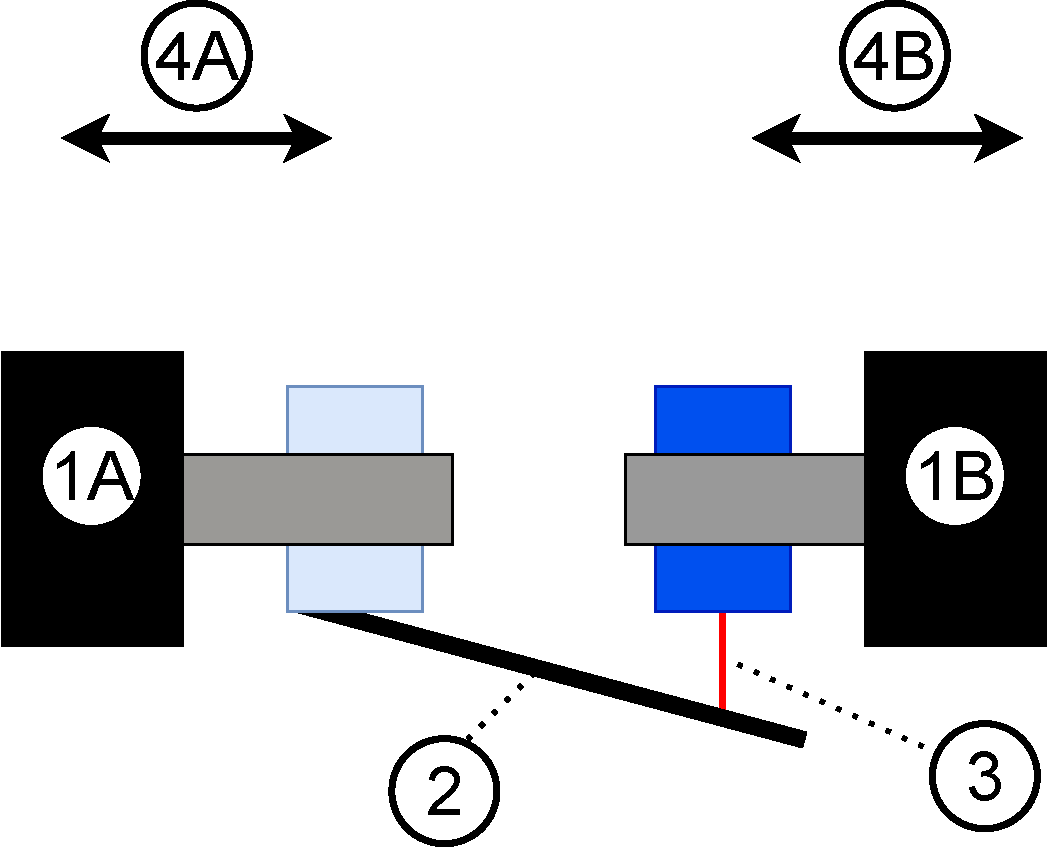
\includegraphics[width=1.2\textwidth]{Figures/c6/schematic_meassurement.pdf}
	   	\caption{Die von Chuy beschriebene und genutzte Plattform.}
	   	\label{K2_chuy_robot_P}
	   \end{subfigure}
	   \hspace{2cm}
	   \begin{subfigure}[b]{0.4\textwidth}
	   	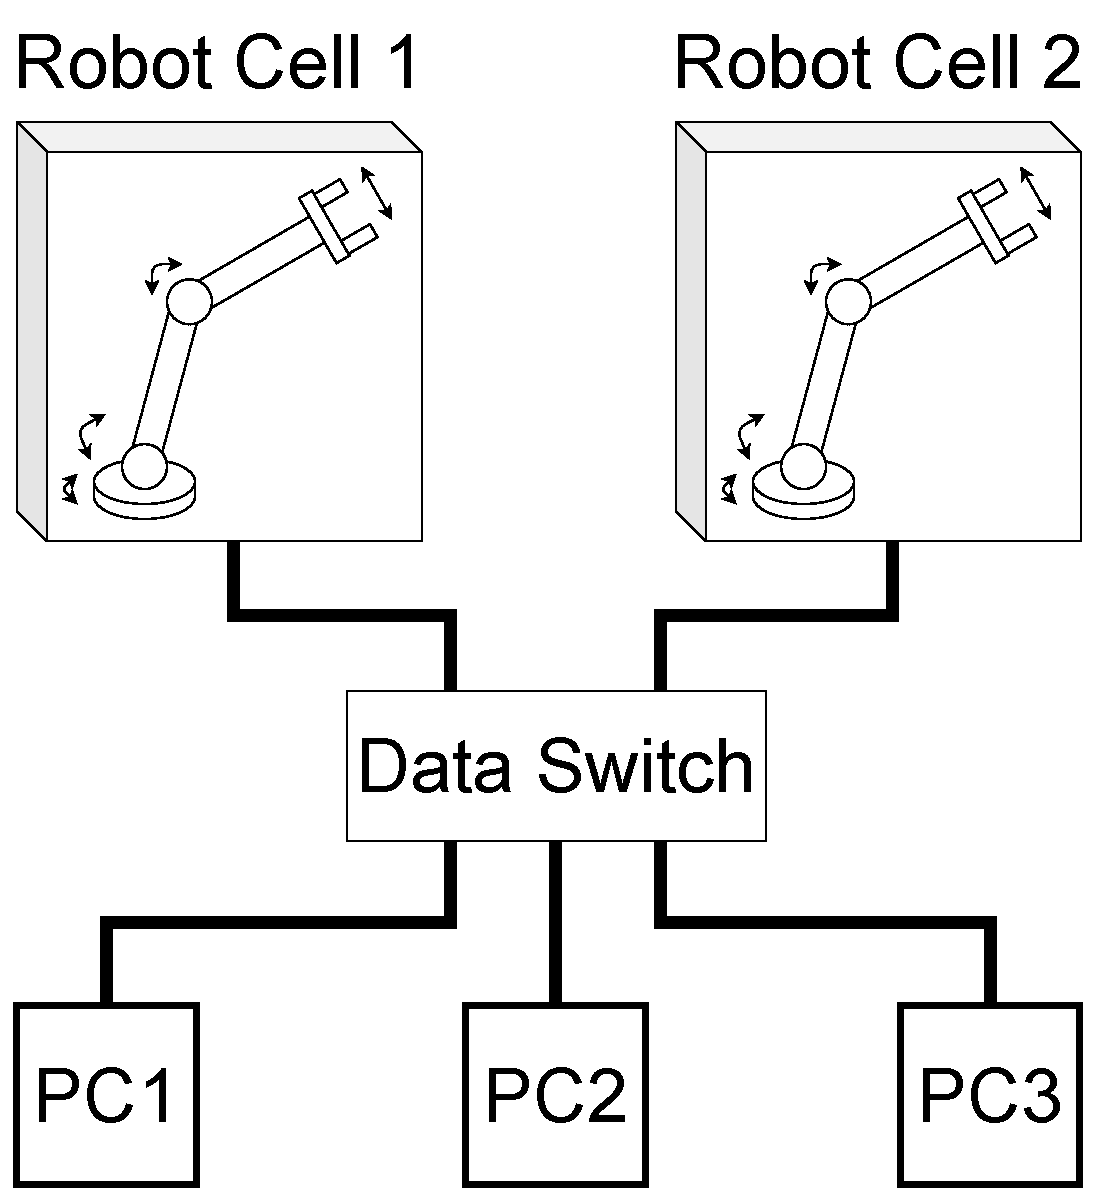
\includegraphics[width=1\textwidth]{Figures/c6/network_setup.pdf}
	   	\caption{Abstrakter Regelungsansatz von Chuy.}
	   	\label{K2_chuy_control_P}
	   \end{subfigure}	
	\caption{Bilder aus \glqq A Control Approach Based on Passive Behavior
		to Enhance User Interaction \grqq{}\cite{chuy_07_approache}}
	\label{K2_chuy_robot_control_P}
\end{figure}

\begin{wrapfigure}{r}{6cm}
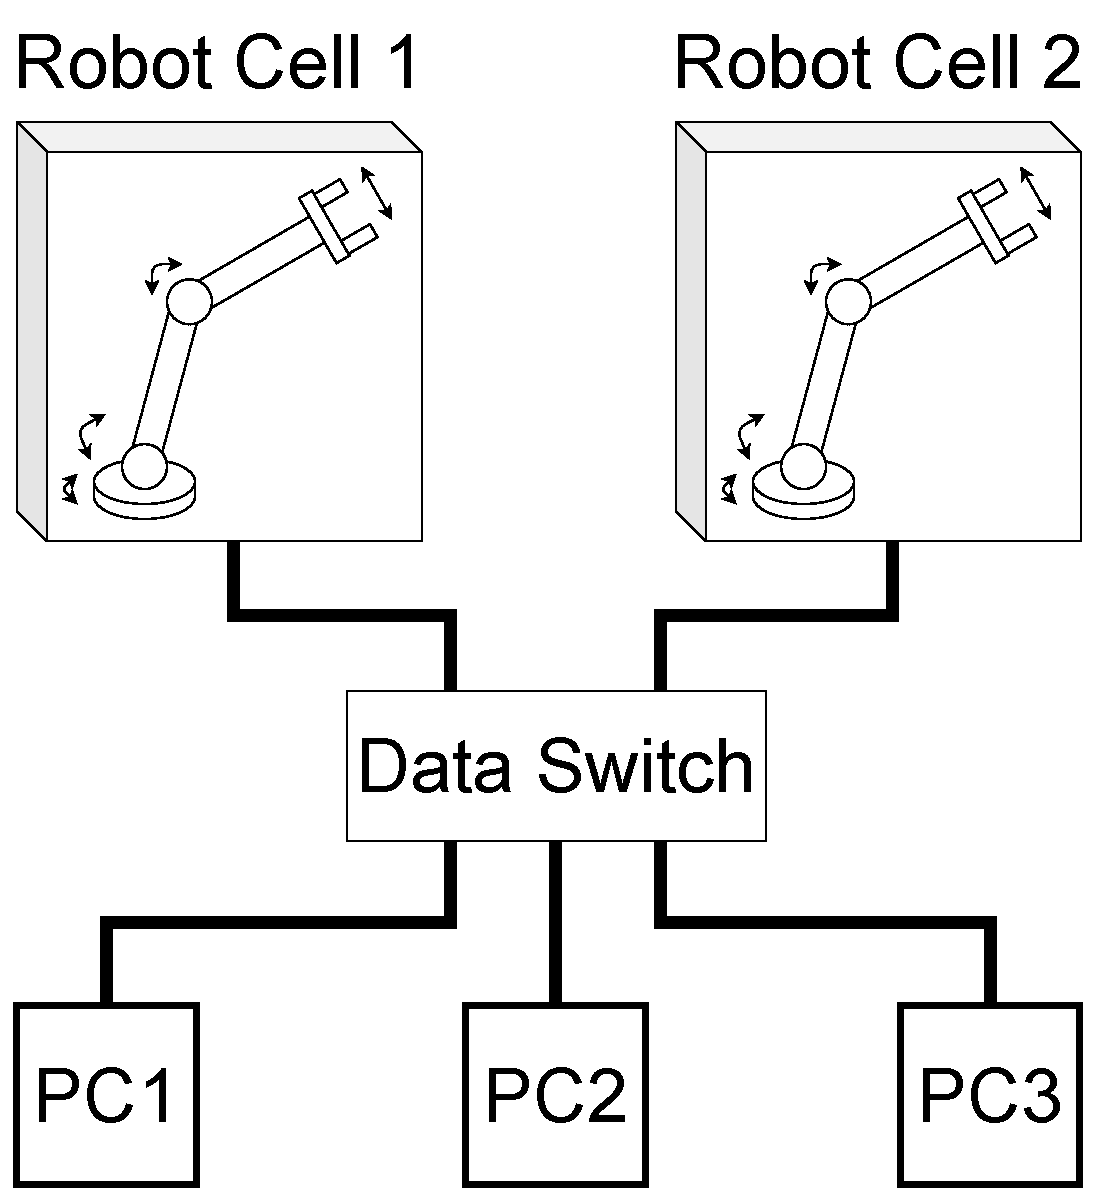
\includegraphics[width=6cm]{Figures/c6/network_setup.pdf}
\caption{Schematic overview of the network setup.} \label{c6_fig_network}
\end{wrapfigure}
\missingfigure{Aufbau}
Add dds parameters, maybe 2-3 settings is enough.
\begin{table}[htbp]
\centering
\begin{tabular}{|l|l|l|l|}
    \hline
Factor & Count & Who & Cite \\\hline
   QoS &     &  &    \\\hline
       &     &   &   \\\hline
       &     &   &   \\\hline
       &     &   &   \\\hline
       &     &   &   \\\hline
       &     &   &   \\\hline
\end{tabular}
\end{table}

\begin{table}[htbp]
    \centering
\begin{tabular}{|l|l|l|l|}
    \hline
Factor & Count & Who & Cite \\\hline
   QoS: sensor profile     &     &  &    \\\hline
       &     &   &   \\\hline
       &     &   &   \\\hline
       &     &   &   \\\hline
       &     &   &   \\\hline
       &     &   &   \\\hline
       
\end{tabular}
\end{table}

Different middlewares:
\begin{enumerate}
    \item Eclipse Cyclone DDS
    \item eProsima Fast DDS
    \item Zenoh
\end{enumerate}
Different Publishing types
\begin{enumerate}
    \item Node topology
    \item Publish trigger
    \item Publish type 
\end{enumerate}

\begin{table}[]
\begin{tabular}{cl|lll}
\multicolumn{1}{l}{}                                  &                                                          & \multicolumn{3}{c}{Middleware}                                                                                \\ \cline{3-5} 
\multicolumn{1}{l}{}                                  &                                                          & \multicolumn{1}{c|}{Eclipse Cyclone DDS} & \multicolumn{1}{c|}{eProsima Fast DDS} & \multicolumn{1}{c}{Zenoh} \\ \hline
\multicolumn{1}{c|}{\multirow{2}{*}{Node topology}}   & \multicolumn{1}{c|}{One node per sub-controller manager} & \multicolumn{1}{l|}{}                    & \multicolumn{1}{l|}{}                  & \multicolumn{1}{l|}{}     \\ \cline{2-5} 
\multicolumn{1}{c|}{}                                 & One node per interface                                   & \multicolumn{1}{l|}{}                    & \multicolumn{1}{l|}{}                  & \multicolumn{1}{l|}{}     \\ \hline
\multicolumn{1}{c|}{\multirow{2}{*}{Publish trigger}} & Publish on timer                                         & \multicolumn{1}{l|}{}                    & \multicolumn{1}{l|}{}                  & \multicolumn{1}{l|}{}     \\ \cline{2-5} 
\multicolumn{1}{c|}{}                                 & Publish on value change                                  & \multicolumn{1}{l|}{}                    & \multicolumn{1}{l|}{}                  & \multicolumn{1}{l|}{}     \\ \hline
\multicolumn{1}{c|}{\multirow{2}{*}{Publish type}} & Normal publisher                                         & \multicolumn{1}{l|}{}                    & \multicolumn{1}{l|}{}                  & \multicolumn{1}{l|}{}     \\ \cline{2-5} 
\multicolumn{1}{c|}{}                                 & Real-time publisher                                      & \multicolumn{1}{l|}{}                    & \multicolumn{1}{l|}{}                  & \multicolumn{1}{l|}{}     \\ \hline
\end{tabular}
\end{table}

\todoin{should probably test with different network workloads...}
\subsection{Hardware}
\paragraph{Robot Platforms}
RSI used for communication with the robots
\paragraph{Computer}
\paragraph{Network}
\begin{figure}[htbp]
	\centering
	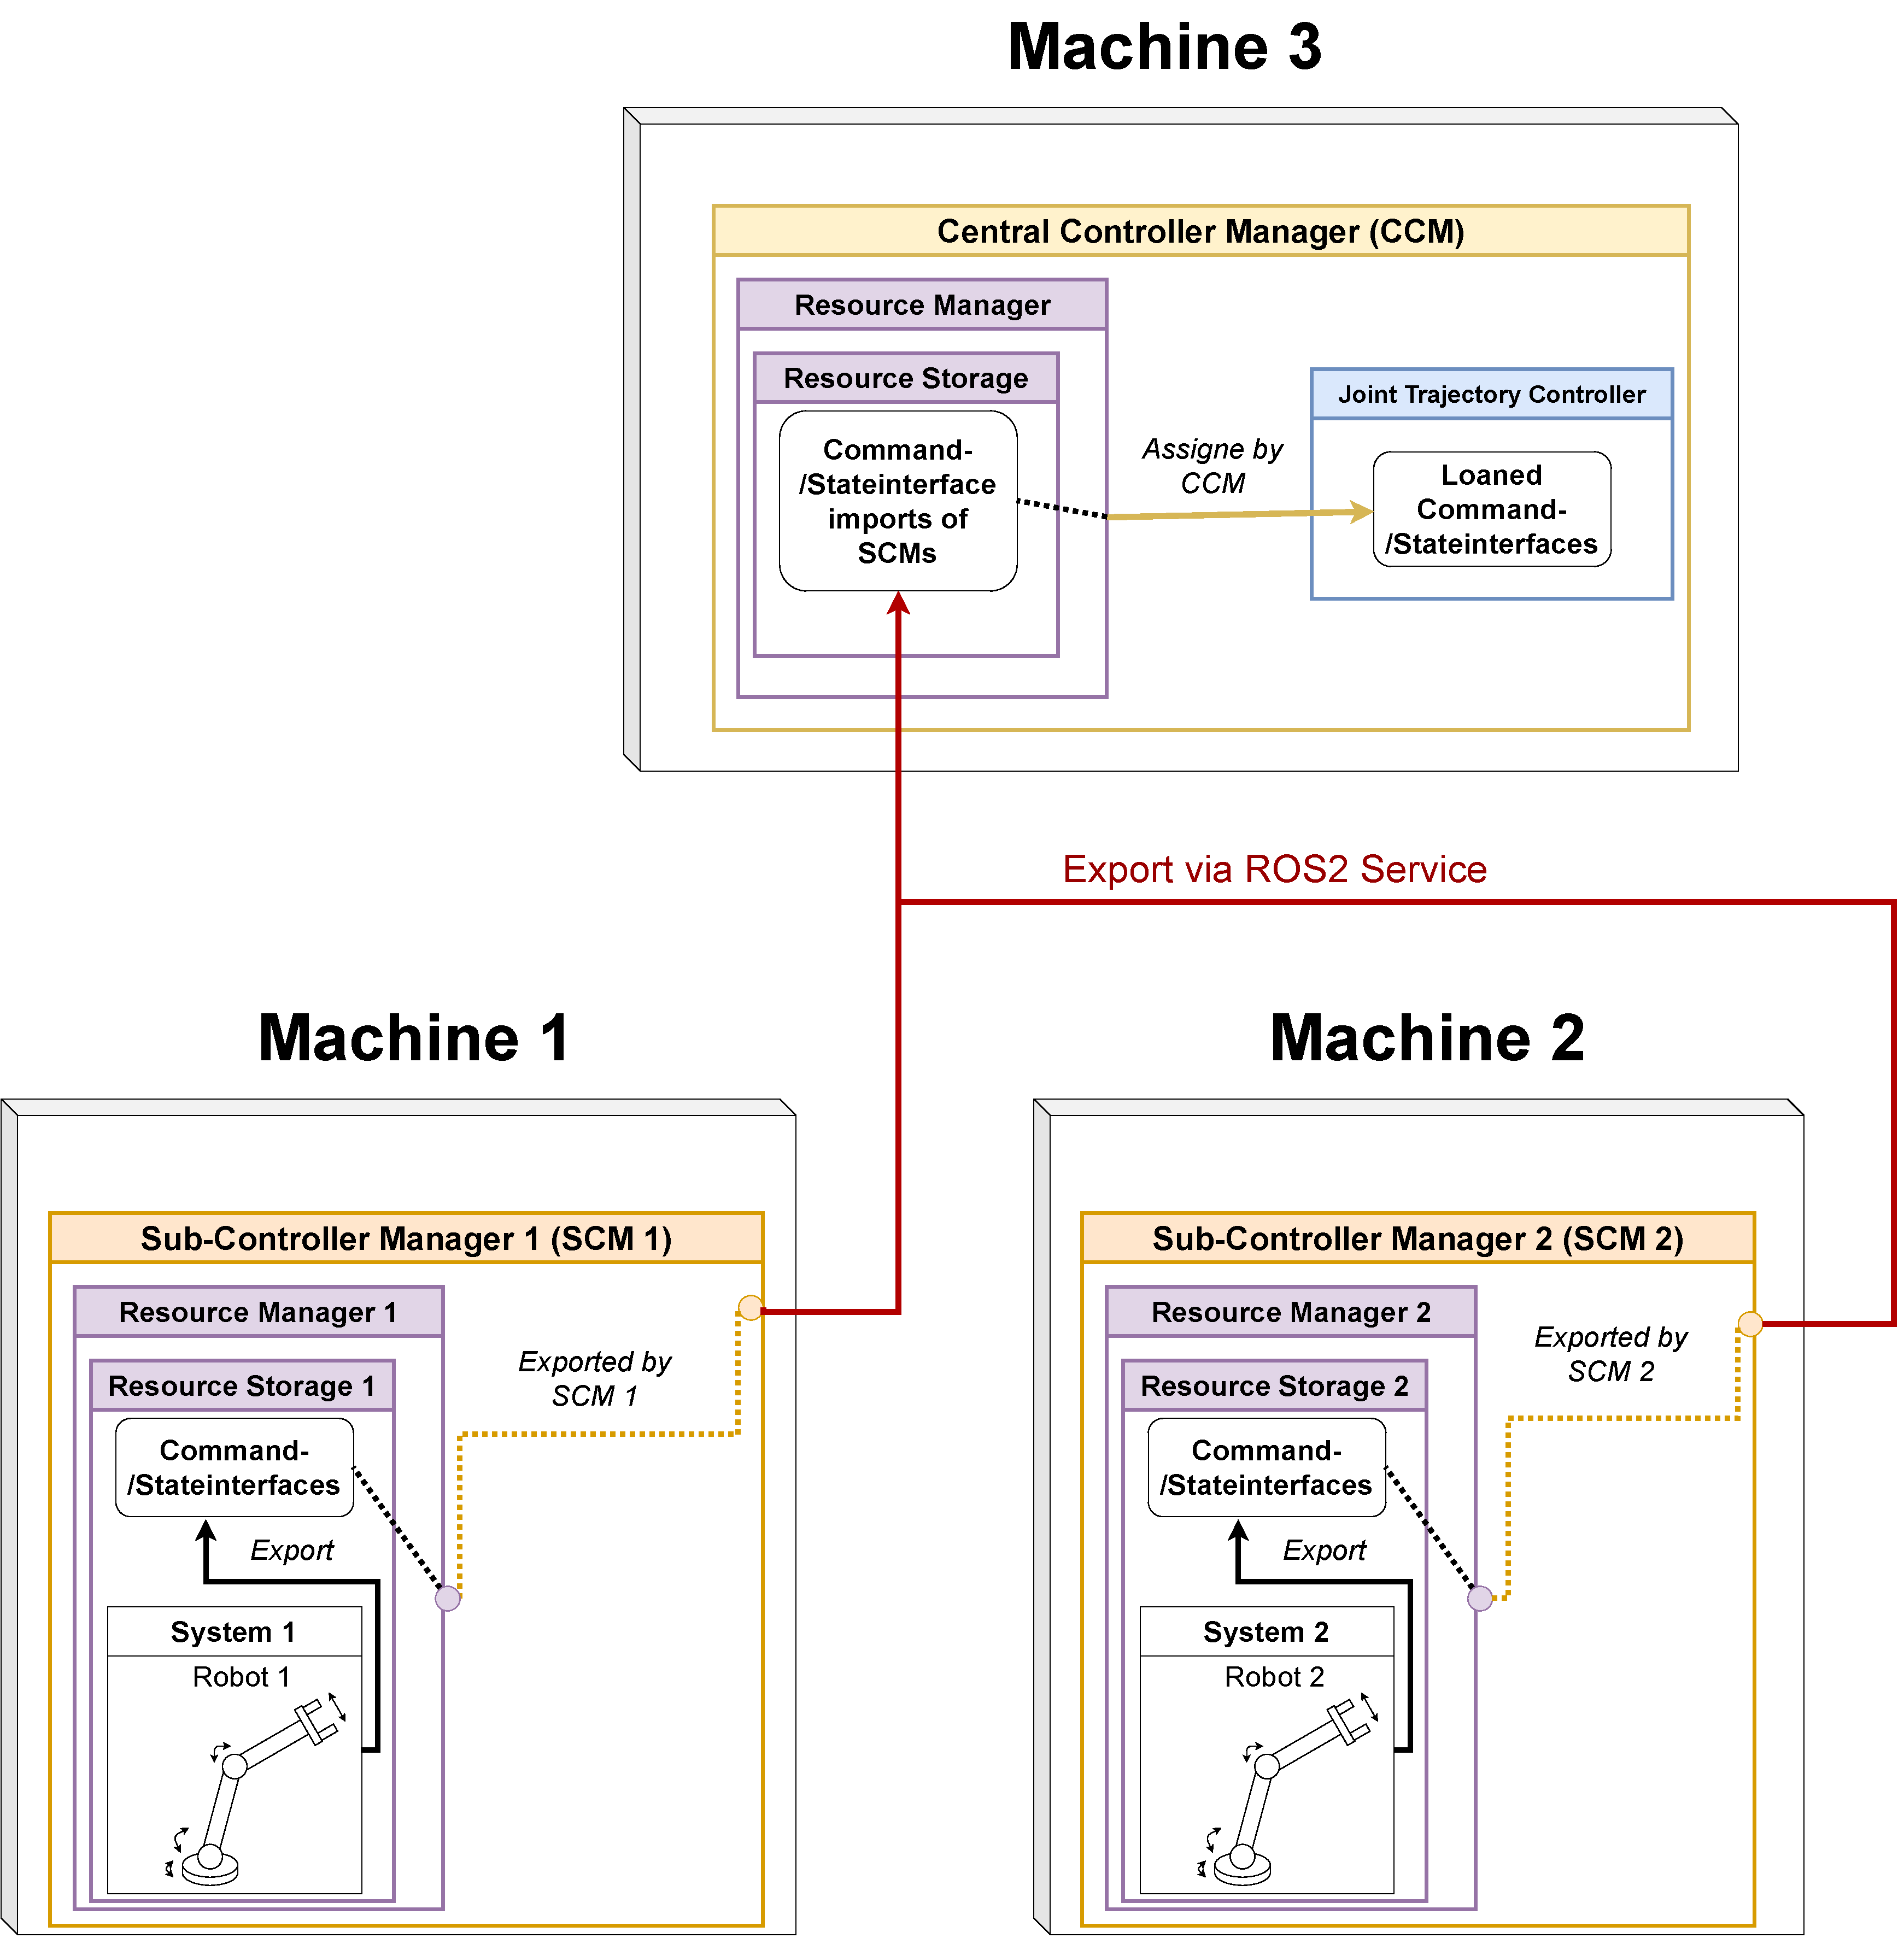
\includegraphics[width=1\textwidth]{Figures/c6/test_scenario_1.drawio.pdf}
	\caption{Schematic overview of the conceptual design of the system for the first test.}
	\label{c6_fig_test_scenario_1}
\end{figure}
\todo{add driver}
\begin{figure}[htbp]
	\centering
	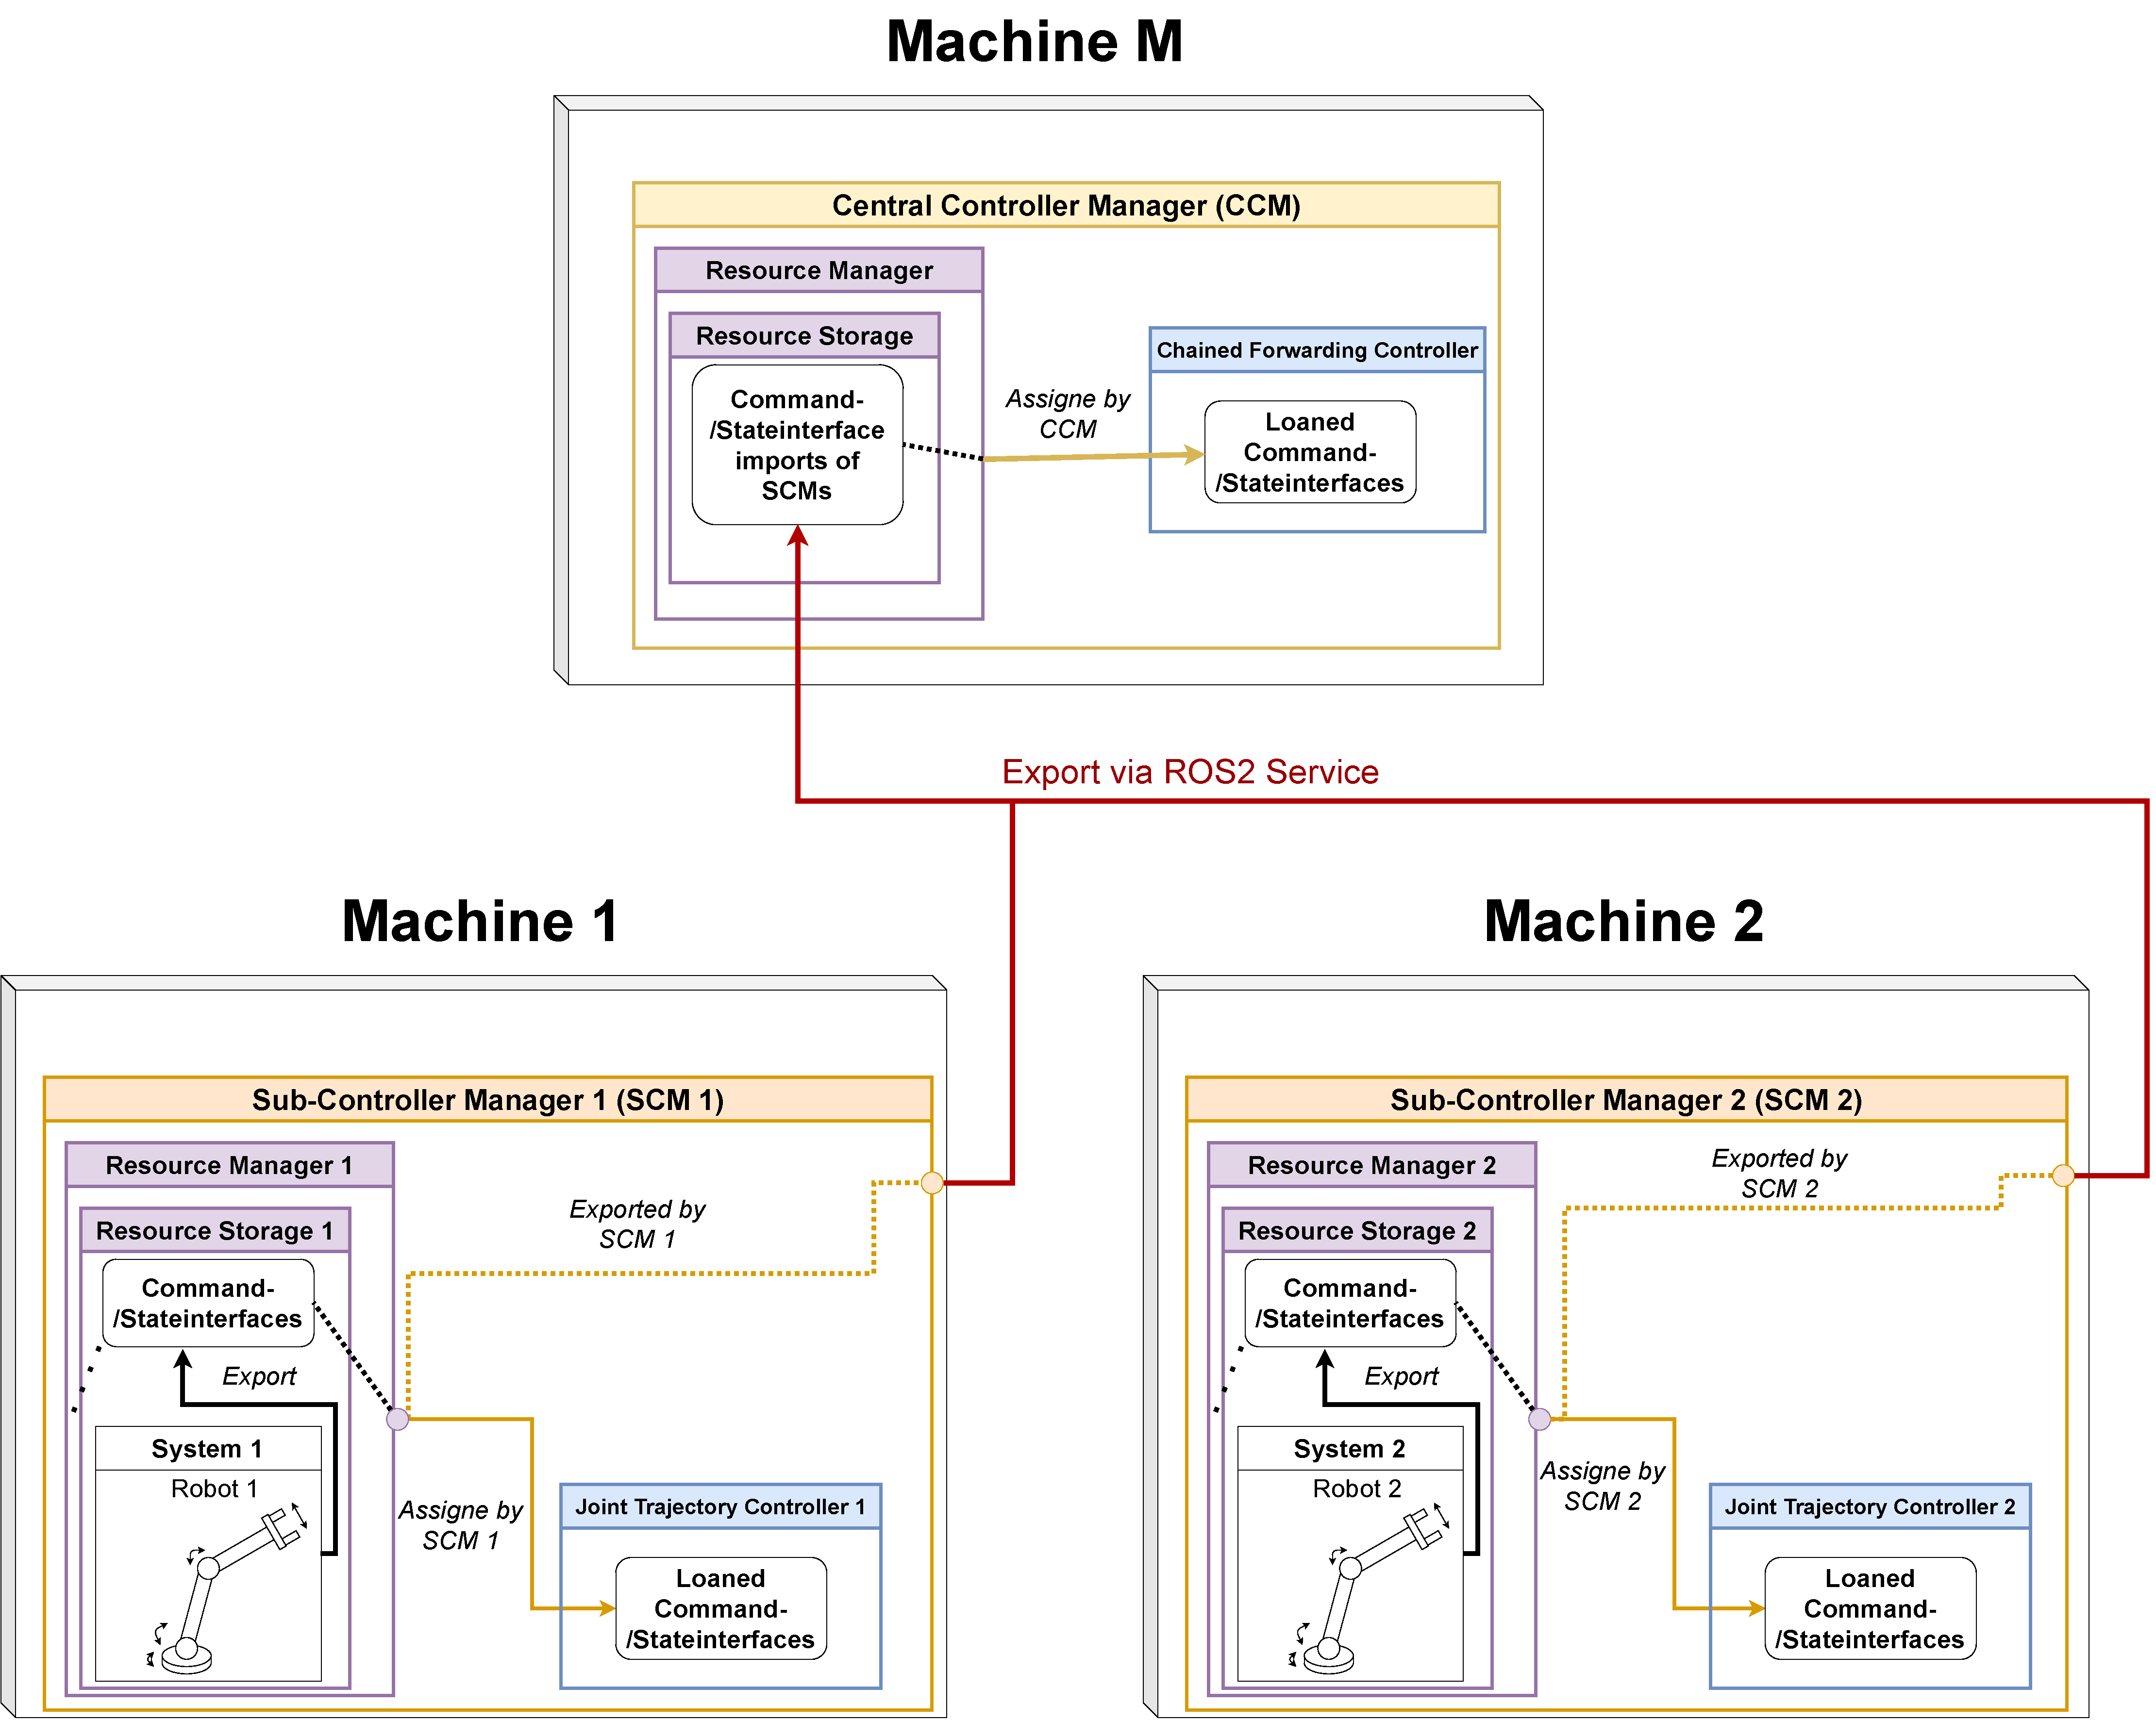
\includegraphics[width=1\textwidth]{Figures/c6/test_scenario_2.drawio.pdf}
	\caption{Schematic overview of the conceptual design of the system for the second test.}
	\label{c6_fig_test_scenario_2}
\end{figure}
\todo{change m to 3}
\todo{add driver}
\section{Distance Sensor}
\subsection{Experimental Setup}
Describe Sensor mount and robot placement.
\missingfigure{Please add some figures}
\subsection{Distributed Drivers}
\subsection{Chained Controllers}
\section{Force Torque Sensor}
\subsection{Experimental Setup}
Describe Sensor mount and robot placement.
\missingfigure{Please add some figures}
\subsection{Distributed Drivers}
\subsection{Chained Controllers}
\section*{Side Note}
Concept has also been tested on KUKA KR 16-2 KUKA KR 5 but because of how they are placed evaluation setup could not be conducted.

